\documentclass[parskip=full]{scrartcl}

\pdfoutput=1

\title{Small Data Oversampling  \\ \LARGE{Improving small data prediction accuracy using the Geometric SMOTE algorithm}}

\author{
	Georgios Douzas\(^{1}\), Fernando Bacao\(^{1}\), Maria Lechleitner\(^{1*}\) 
	\\
	\small{\(^{1}\)NOVA Information Management School, Universidade Nova de Lisboa}
	\\
	\small{*Corresponding Author}
	\\
	\\
	\small{Postal Address: NOVA Information Management School, Campus de Campolide, 1070-312 Lisboa, Portugal}
	\\
	\small{Telephone: +351 21 382 8610}
}

\usepackage{breakcites}
\usepackage{float}
\usepackage{graphicx}
\usepackage{geometry}
\usepackage[colorinlistoftodos]{todonotes}
\geometry{
	a4paper,
	total={170mm,257mm},
	left=18mm,
	right=18mm,
	top=18mm,
}
\usepackage{amsmath}
\newcommand{\inlineeqnum}{\refstepcounter{equation}~~\mbox{(\theequation)}}
\usepackage{enumitem}
\usepackage[ruled,vlined]{algorithm2e}
\usepackage{booktabs}
\usepackage{pgfplotstable}
\pgfplotsset{compat=1.14}
\usepackage{longtable}
\usepackage{tabu}
\usepackage{hyperref}
\usepackage{csvsimple}
\usepackage{graphicx}
\usepackage{adjustbox}
\usepackage{longtable}
\usepackage{caption}
\date{}

\begin{document}

\maketitle

\begin{abstract}
Small training datasets decrease the performance of machine learning algorithms
which results in poor analysis and decision making. The current research work
aims to investigate the effect of using small datasets and provide a solution by
artificially adding samples in the training process. More specifically, the
over-sampling technique Geometric SMOTE is applied to generate new instances and
enhance the initial training data. The experimental results show a significant
improvement on the prediction capability when comparing with other over-sampling
techniques such as Random Oversampling, SMOTE and Borderline SMOTE. These
findings create a linkage between the research areas of the imbalance learning
problem and the small data problem which offers a lot of potential for future
research.
\end{abstract}

\section{Introduction}
One of the key problems in supervised learning is the insufficient size of data
sets \cite{Niyogi.1998}, \cite{AbdulLateh.2017}. The limited availability of
training samples can be caused by different factors. First, data is becoming an
increasingly expensive resource \cite{Li.2007} as the process to retain data is
getting more complex due to strict privacy regulations such as the General Data
Protection Regulation (GDPR) \cite{EuropeanCommission.2019}. Additionally, the
small dataset problem can be found in numerous industries where organizations
simply do not have access to a reasonable amount of data. For example, manufacturing 
industries are usually dealing with small data in early stages of
product developments and health care organizations have to work with different
kinds of rare diseases, where very few records are available \cite{AbdulLateh.2017}.

In machine learning, researchers are mainly concerned with the design of 
sophisticated learning algorithms when aiming to improve prediction 
performance. However, the more successful way is often to increase the sample 
size. Domingos states a rule of thumb that "a dumb algorithm with lots and lots 
of data beats a clever one with modest amounts of it" \cite{Domingos.2012}. One 
of the reasons why the application of refined algorithms does not perform well 
on an insufficient amount of data is that small data often does not provide an 
unbiased representation of reality. Small sample sets are characterized by a 
loose data structure with many information gaps whereas a bigger dataset 
carries more observations to provide a complete picture of the problem. This 
lack of learning information negatively impacts the performance of the machine 
learning algorithms \cite{Lin.2018}. Consequently, the knowledge gained from 
prediction models trained with small sample sizes is considered unreliable as 
well as imprecise and does not lead to a robust classification performance 
\cite{AbdulLateh.2017}.

Considering the size of data, there are two types of problems: first, the 
insufficiency of data belonging to one class (imbalance data problem) and 
second, the size of the whole data (small dataset problem) \cite{Sezer.2014}. 
In both cases, a small training sample set does not provide enough information 
to a machine learning model to obtain a stable learning accuracy 
\cite{Tsai.2008}. A theoretical explanation of “small” can be found in 
statistical learning theory by Vapnik. A sample size is defined as small, if 
the ratio between the number of training samples and Vapnik-Chervonenkis (VC) 
dimensions is less than 20. Where VC dimensions are determined as the maximum 
number of vectors that can be separated into two classes in all possible ways 
by a set of functions \cite{Vapnik.2008}. 

Under-representation of observations in the sample set, the small dataset 
problem, can be solved in different ways. The use of synthetic data derived 
from existing (real) observations is a promising approach to the problem 
\cite{Sezer.2014}. As a result, techniques to artificially add information by 
extending the sample size, and eventually improving the classification results 
of the algorithms, can translate into significant improvements in many 
application domains. However, it is important to consider that virtual data 
samples are not necessarily representatives of the population, as they are 
artificially created. Taking this into consideration, the challenge in 
artificial data generation is to create data which extends the observed data 
without creating noise \cite{Li.2006}. Additionally, it is important to 
consider that generating artificial data will only work if the available sample 
is representative of the underlying population.

\begin{figure}[H]
	\centering
	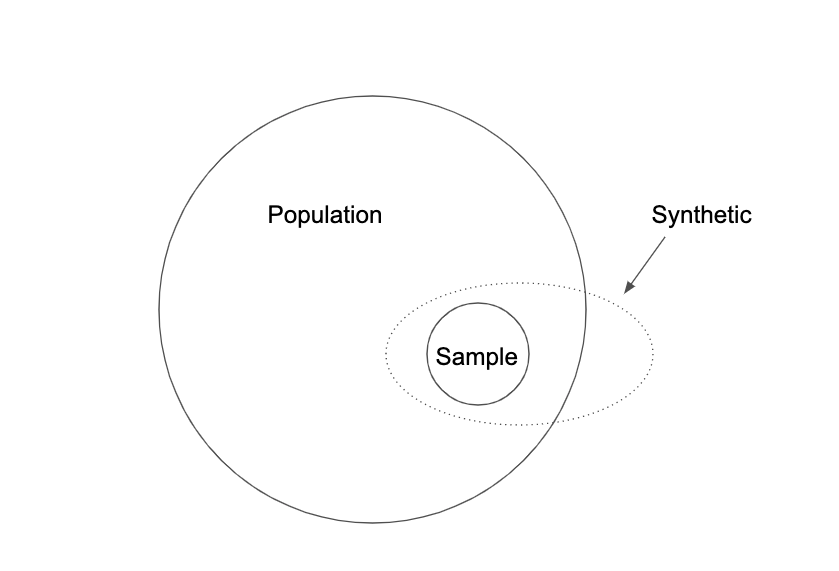
\includegraphics[width=0.35\linewidth]{./resources/relationship}
	\caption{Relationship between population, actual data and virtual data \cite{Li.2006}}
	\label{fig:relationship}
\end{figure}

The next sections will describe an effective way to tackle the small dataset 
problem. In chapter 2, the previously studied solutions are reviewed. Next, a 
detailed description of the proposed method is presented in chapter 3. This is 
followed by the research methodology and the experimental results in chapter 4 
and 5. Finally, the paper is concluded with an analysis of the experiments in 
chapter 6.

\section{Related Work}
Several data pre-processing methods to increase the data size have been
presented by the research community. In this section, the most important
approaches are reviewed and the state-of-the-art to improve small dataset
learning is reported. We start by presenting fuzzy theories, which have 
historically been the most used approach to mitigate the small dataset problem. 
Next, we look at resampling mechanisms, which mainly consist of bootstrapping 
techniques, and finally, we review over-sampling techniques that can be a 
valuable option to increase the sample size in small datasets.

\subsection{Fuzzy Theories}

One of the most effective methods to improve the learning performance of 
prediction models is artificial sample generation. It has been shown that the 
accuracy of the learning algorithm is improved, when the sample size of 
training sets is increased \cite{AbdulLateh.2017}. Thus, the objective is to 
fill the gaps between observations (information gaps) with synthetic samples 
that are derived from the original population to feed the algorithm with a more 
complete representation of the reality.

\begin{figure}[H]
	\centering
	\includegraphics[width=0.6\linewidth]{"./resources/small_data_distribution"}
	\caption{Distribution of a small dataset \cite{Tsai.2015}}
	\label{fig:small-data-distribution}
\end{figure}

Many techniques presented in the literature are based on fuzzy theories
\cite{AbdulLateh.2017}. The fuzzy set theory provides a strict mathematical
framework to generalize the classical notion of a dataset. It gives a wider
scope of applicability, especially in the fields of information processing and
pattern classification \cite{Zimmermann.2010}. Based on this concept, several
methods have emerged in the last decade to estimate or approximate functions
which are generating more samples for sparse training sets.

The fundamental concept of artificially creating data is called Virtual Sample 
Generation (VSG) and was originally proposed by \cite{Niyogi.1998}. The idea is 
to create additional examples based on the current set of real-life examples by 
using prior information gained from the available data. The introduction of 
virtual examples expands the effective training set size and can therefore help 
to mitigate the learning problem. \cite{Niyogi.1998} showed that the process of 
creating artificial samples is mathematically equivalent to incorporating prior 
knowledge. They demonstrate the concept on object recognition by mathematically 
transforming the views of 3D-objects. These new views are called ‘virtual 
samples’ and its application extends information and results in successful 
generalization. 

Based on this theory, several closely related studies were developed for
manufacturing environments. The first method to overcome scheduling problems due
to the lack of data in early stages of manufacturing systems was the creation of
a Functional Virtual Population (FVP) \cite{Li.2003}. The idea is to
create a number of virtual samples within of a newly defined domain range. The
method involves a highly manual process, however, the application of FVP
dramatically improved the classification accuracy of a Neural Network. 

In 2004, the idea of fuzzifying information to extend a small dataset was used 
to develop the Diffusion-Neural-Network (DNN) method \cite{Huang.2004}. It 
combines the principle of information diffusion by \cite{Huang.1997} with 
traditional Neural Networks to estimate functions. The information diffusion 
method partially fills the information gaps by using fuzzy theories to 
represent the similarities between samples and subsequently derive new samples. 

The researchers \cite{Li.2006b} further examined possible methods to learn
scheduling knowledge with rare data in early stages of manufacturing systems.
They developed a new data fuzzification technique called mega-fuzzification and
combined it with a data trend estimation procedure to systematically expand the
small dataset. The method fuzzifies the dataset as a whole and expands it in
consideration of a previously defined data trend. The results of this study 
show high learning accuracy and denote the method as a reliable and applicable 
approach in the business marketplace. However, the difficulty in establishing 
the domain ranges and the lack of a theoretical basis explain its lack of 
popularity and limited interest. 

In order to fully fill the information gaps, a technique which diffuses the
sample set one for one was introduced by \cite{Li.2007}. Their concept is to 
combine data trend estimation with a diffusion technique to estimate the domain 
range mainly to avoid over-estimation. The method is called 
Mega-Trend-Diffusion (MTD) and diffuses a set of data instead of each sample
individually. For example, two samples $\mathit{m}$ and $\mathit{n}$ (Figure 3) 
are diffused simultaneously into one function with their borders $\mathit{a}$ 
and $\mathit{b}$. To estimate $\mathit{a}$ and $\mathit{b}$, the algorithm takes
the minimum and maximum values of the dataset and counts the number of data 
points which are smaller or greater than the average of the values. This takes 
the skewness in the distribution of the data and the domain range into 
consideration when calculating new samples. The triangular shape of Figure 3 
represents the membership function which shows the similarities between 
samples. $\mathit{M}$ and $\mathit{n}$ are the samples and their heights are 
the possible values of the membership function.

\begin{figure}[H]
	\centering
	\includegraphics[width=0.6\linewidth]{"./resources/mtd_function"}
	\caption{MTD function \cite{Li.2007}}
	\label{fig:mtd-function}
\end{figure}

After estimating the domain range between $\mathit{a}$ and $\mathit{b}$, 
samples are randomly produced within this area by using a common diffusion 
function. The artificial samples are then trained with a Back-propagation 
Neural Network (BPNN) like \cite{Huang.2004} originally proposed. This 
technique is seen as an improvement of DNN and was initially developed to 
improve early flexible manufacturing system scheduling accuracy. In further 
research, MTD is widely used as a synthetic sample generation method and is 
recognized as an effective way to deal with small dataset problems 
\cite{AbdulLateh.2017}. However, MTD only considers the data for independent 
attributes and does not deal with their relationships. 

Also, a genetic algorithm based virtual sample generation (GABVSG) was 
proposed. The method takes the relationship among the attributes into account 
and explores the integrated effects of attributes instead of dealing with them 
individually. This algorithm is performed in three steps: Samples are randomly 
selected to determine the range of each attribute by using MTD functions. Next, 
a Genetic Algorithm is applied to find the most feasible virtual samples. 
Finally, the average error of these new samples is calculated. The results 
outperformed the ones using MTD and also showed better performance in 
prediction than in case of no generation of synthetic samples \cite{Li.2014}.

The above presented fuzzy-based algorithms are limited on numerical attributes. 
When the dataset contains nominal features, resampling mechanisms have to be 
considered such as Bootstrap. Although it is possible to transform nominal 
values into binary ones, the relationship between the values of the attributes 
would get lost \cite{Tsai.2008}. 

\subsection{Resampling Mechanism}

An alternative approach to fuzzy theories is the Bootstrapping Procedure (BP),
which is the most well-known artificial sample generation method
\cite{AbdulLateh.2017}. The main difference to the previously presented
techniques is that BP creates new training sets by resampling instances from the
measured data with replacement \cite{Efron.1993}. It allows the algorithms to
use the same sample more than one time to gradually revise the identified
patterns in order to improve predictive accuracy. Although this can double the
number of observations from the training sets, Bootstrapping can cause
overfitting when applied to small data because it repetitively uses the same
information. Also, since the amount of information provided by small data is
minimal, any missing observations in the new, bootstrapped training sets are a
loss of valuable information (see Figure 4). As a result, Bootstrap cannot be
seen as a solution to the small dataset problem, as it increases the number of
training samples rather than the amount of (artificially generated) information
\cite{Tsai.2015}, \cite{Li.2018}. However, \cite{Ivanescu.2006} applied BP in
batch process industries where it was shown that it may help mitigate the
limited data problem.

\begin{figure}[H]
	\centering
	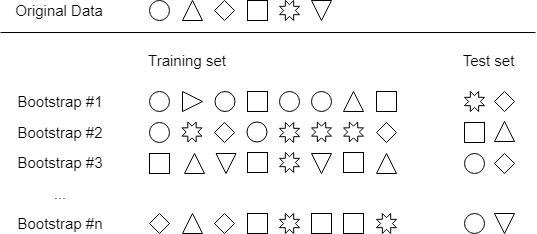
\includegraphics[width=0.6\linewidth]{./resources/bootstrapping_example}
	\caption{Example of bootstrapping sets, where six samples are represented 
	as symbols and are allocated to $\mathit{n}$ possible subsets. The size of 
	the subsets are increased using multiple instances of the original data. 
	The data points which are not selected by the BP are used as a test set 
	\cite{Kuhn.2013}.}
	\label{fig:bootstrappingexample}
\end{figure}

In further studies of \cite{Tsai.2008} and \cite{Chao.2011}, the BP was applied
to actually generate virtual samples in order to fill the information gaps.
Instead of resampling observations, they execute the BP once for each input
factor which results in a newly shuffled training set. After generating new
instances, they are combined with the original dataset to train a Neural
Network. The results show that this method significantly decreases the
prediction error rate in modeling manufacturing systems as well as in the
prediction to radiotherapy of bladder cancer cells.

\subsection{Over-sampling Techniques}

A different approach to fill information gaps is synthetic over-sampling of the
training set. Over-sampling is an artificial data generation strategy originally
developed in the context of machine learning to mitigate the imbalanced learning
problem. Its origin comes from a different research community than the fuzzy
strategies presented above, which is more related to machine learning
techniques. Although over-sampling, fuzzy theories and resampling approaches are
aiming to solve a similar problem, it seems that these communities have had very
few connections so far. 

In the imbalanced learning problem, the classes of the given dataset are
significantly skewed. This means, that the dataset has a large number of
observations in one class and a very small number of observations in the other
class or classes. This constitutes a problem for the algorithm to learn and is
aimed to be solved in the training phase. In practice, the imbalanced dataset
problem is are very common issue in supervised learning. Especially, in the
fields of fraud detection, product categorization and disease diagnosis, an
imbalanced dataset is the norm rather than the exception \cite{He.2013}. 

\subsubsection{SMOTE}

There are several methods presented in the literature to tackle this problem.
The first method to be proposed and still the most popular is the synthetic
minority oversampling technique (SMOTE). SMOTE works based on the idea of
k-nearest neighbors and linear interpolation. More specifically, it forms a line
segment between neighboring minority class instances and and generates synthetic
data between these samples \cite{Chawla.2002}. The algorithm is considered as a
standard selection due to its simplicity
as well as its robustness. Numerous variations have been proposed based on SMOTE
increasing its status as the staple idea in over-sampling for imbalanced learning
problems \cite{Fernandez.2018}. However, SMOTE presents some signifiant
limitations when it comes to the sample generation process. In practice, the
separation between majority and minority class clusters is often not clearly
definable. Thus, noisy samples may be generated when a minority sample lies in
the region of the majority classes. Figure 5 presents a scenario where a
minority instance is generated within the majority region (noisy sample).

\begin{figure}[H]
	\centering
	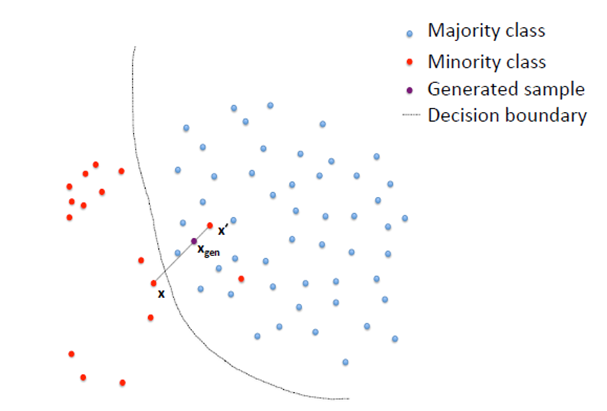
\includegraphics[width=0.6\linewidth]{./resources/noisy_examples}
	\caption{Generation of noisy examples \cite{Douzas.2019b}}
	\label{fig:noisy-examples}
\end{figure}

Furthermore, redundant instances may be generated within dense minority 
regions, as so that they do not add any relevant information to the classifier 
and may lead to overfitting. Figure 6 demonstrates an example where a minority 
class instance is generated in a dense minority class. This new observation 
belongs to the same dense cluster as the original and is therefore less useful. 

\begin{figure}[H]
	\centering
	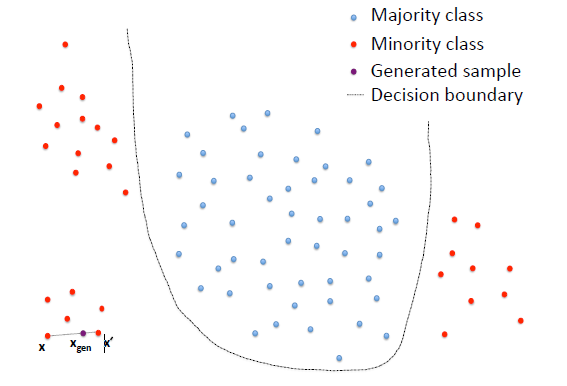
\includegraphics[width=0.6\linewidth]{./resources/redundant_examples}
	\caption{Generation of redundant examples \cite{Douzas.2019b}}
	\label{fig:redundant-examples}
\end{figure}

Although SMOTE is recognized as a oversampling technique for imbalanced
datasets, it can also be used for solving the small dataset problem. 
\cite{Li.2018} proved that SMOTE is able to successfully fill the information 
gaps with synthetic samples. However, given its limitations, it did not achieve 
the best results within their study.

\subsubsection{G-SMOTE}

The novel data generation procedure Geometric SMOTE (G-SMOTE) has been 
presented with the objective to improve the above mentioned limitations of the 
SMOTE algorithm \cite{Douzas.2019b}. G-SMOTE can be seen as a substitute of 
SMOTE enhanced by geometric properties. The main difference to SMOTE is that 
it broadens the options for data generation and 
prevents the creation of noise. Instead of connecting the minority sample and one of 
its nearest neighbors with a line segment, the instances are 
generated in a geometrical region (hyper-spheroid) around the minority sample. 
Furthermore, G-SMOTE is designed to avoid the generation of noisy samples by 
some restrictions in the selection strategy. Figure 7 demonstrates the 
distribution of artificially created samples by SMOTE versus G-SMOTE. With an 
increased number of $\mathit{k}$ neighbors, SMOTE tends to generate noisy 
samples, whereas Geometric SMOTE avoids this scenario.

\begin{figure}[H]
	\centering
	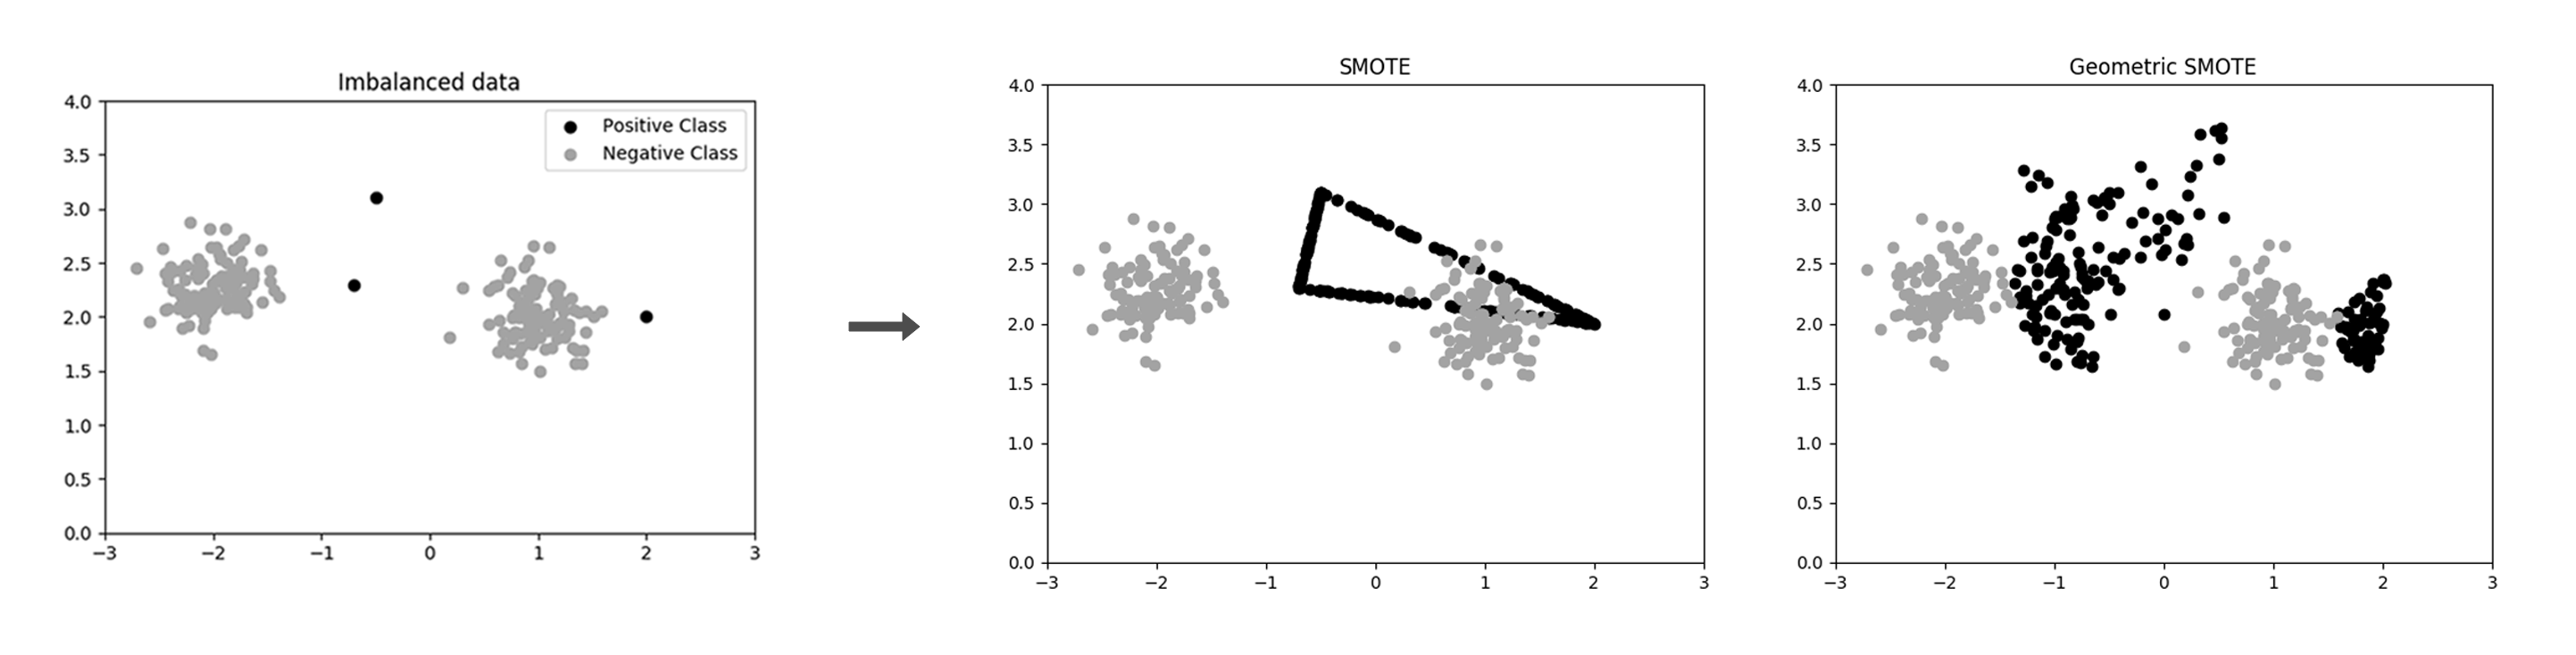
\includegraphics[width=1\linewidth]{./resources/smote_vs_gsmote}
	\caption{SMOTE versus G-SMOTE \cite{Douzas.2019}}
	\label{fig:smotevsgsmote}
\end{figure}

The study of \cite{Douzas.2019b} has performed an extensive comparison between 
G-SMOTE and SMOTE using 69 imbalanced datasets and several classifiers. The 
results show that G-SMOTE outperforms SMOTE, Random Oversampling and the case 
of no oversampling, across all datasets, classifiers and performance 
metrics.    

Various methods to deal with small datasets or a small representation 
within a class label have been presented in this section. It has been proven, 
that all cases with artificially increased sample size seem to enhance the 
prediction performance of the classifier. Thus, we can conclude 
that increasing the sample size of a small or imbalanced dataset is an 
important task in the area of machine learning \cite{Ruparel.2013}. However, 
most of the studied methods are associated with a lot of limitations and are 
not easy to understand. Considering these methods in practice, an application 
has still been challenging \cite{Sezer.2014}. As a result, we propose a 
different approach to overcome the issues sourced form the absence of data and 
provide a framework for an easy implementation of the algorithm.

\section{Proposed Method}

In the following section, we propose G-SMOTE as a novel data generation procedure 
for small datasets. Originally developed for imbalanced datasets, we 
slightly adapt the algorithm to not only increase the minority class, but the 
entire dataset independent from class occurrences. 

\subsection{G-SMOTE for the small dataset problem}

As mentioned above, the G-SMOTE algorithm randomly generates artificial data
within a geometrical region of the input space. The size of this area is derived
from the distance of the selected sample to one of the nearest neighbors,
whereas the shape is determined by the hyper-parameters called as truncation
factor and deformation factor. Additionally, the hyper-parameter selection
strategy of G-SMOTE modifies the SMOTE selection process. The main concept can
be adapted from the original method to the small dataset problem. However, the
selection strategy requires some minor adjustments for these kind of problems
which will be described hereafter.

The selection strategy $\alpha$\textsubscript{sel} determines the data points 
of the $\mathit{k}$ nearest neighbors. This mechanism allows the positive or 
negative class area to expand into a direction where it prevents the algorithm 
from creating noisy samples. In G-SMOTE for small data both classes are 
selected in two individual runs to introduce new observations. In the first 
run, a random sample called x\textsubscript{surface} is selected which belongs 
to the positive class. Similarly, x\textsubscript{surface} is assigned to the 
negative class samples in the second run. Both runs are based on the defined 
selection strategy where $\alpha$\textsubscript{sel} can have three different 
values: positive class selection S\textsubscript{pos}, negative class selection 
S\textsubscript{neg} and combined selection S\textsubscript{com}. We describe 
the cases referring to first run of randomly selecting a positive sample. In 
the second run, a negative class example is randomly chosen and the process is 
repeated reversely. 

\begin{enumerate}[label=($\alph*$)]

\item Positive class selection

With the hyperparameter selection\_strategy = 'positive', a second positive 
class sample is selected as one of the $\mathit{k}$ nearest neighbors. This 
indicates that the selection strategy is based only on the positive class and 
works like the selection strategy of SMOTE. As SMOTE may lead to the generation 
of data penetrating the opposite class area, this drawback also applies on the 
selection strategy here.

\begin{figure}[H]
	\centering
	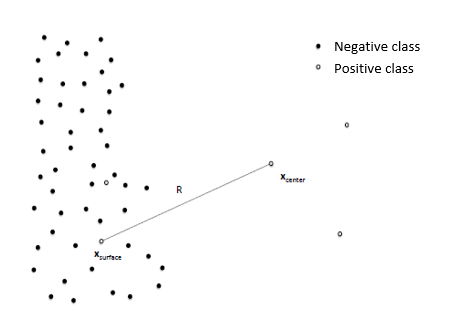
\includegraphics[width=0.51\linewidth]
		{./resources/positive_class_selection_strategy}
	\caption{Example of positive class selection strategy: A positive class 
	instance is defined as the center and one of its $\mathit{k = 4}$ positive 
	class nearest neighbors is selected as the surface point. The radius 
	$\mathit{R}$ is equal to the distance of these instances 
	\cite{Douzas.2019b}.}
	\label{fig:positiveclassselectionstrategy}
\end{figure}

\item Negative class selection

When selection\_strategy = 'negative', a negative sample is selected as the 
nearest class neighbor. This scenario prevents the algorithm from creating 
noisy samples. More specifically, as the radius is drawn from the selected 
positive class instance to the nearest neighbour of the negative class, it does 
not allow the data generation mechanism to penetrate the opposite area.

\begin{figure}[H]
	\centering
	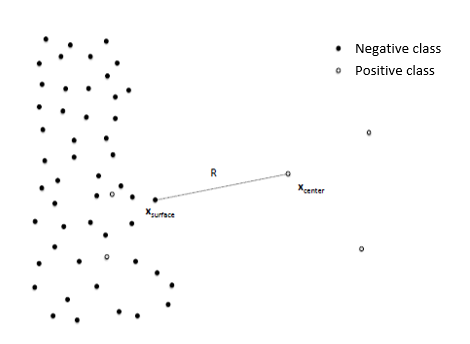
\includegraphics[width=0.5\linewidth]
		{./resources/negative_class_selection_strategy}
	\caption{Example of negative class selection strategy: A positive class 
	instance is defined as the center and its closest negative class neighbor 
	is selected as the surface point. The radius $\mathit{R}$ is defined to be 
	equal to the distance of these instances \cite{Douzas.2019b}.}
	\label{fig:negativeclassselectionstrategy}
\end{figure}

\item Combined selection

The combined selection strategy initially applies the positive and negative 
selection strategies. Once x\textsubscript{pos} and x\textsubscript{neg} are 
identified, the point with the minimum distance to the center 
x\textsubscript{center} is defined as the surface point 
x\textsubscript{surface}. Figure 10 presents an example when 
x\textsubscript{surface} is identified as a negative class instance.

\begin{figure}[H]
	\centering
	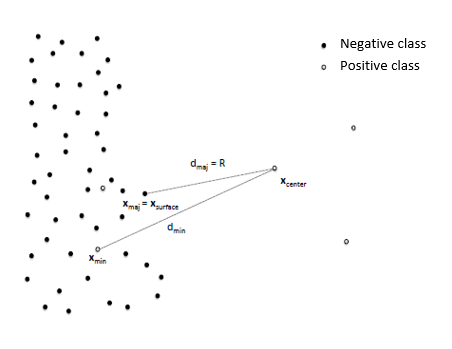
\includegraphics[width=0.52\linewidth]
		{./resources/combined_class_selection_strategy}
	\caption{The closest point x\textsubscript{neg} to the center positive 
	class sample x\textsubscript{center} is identified as the surface point 
	x\textsubscript{surface} since it is closer to the center than the 
	selected instance x\textsubscript{pos} from the $\mathit{k}$ nearest 
	positive class neighbors of the center \cite{Douzas.2019b}.}
	\label{fig:combinedclassselectionstrategy}
\end{figure}

\end{enumerate}

%More adjustments?

\subsection{Adapted G-SMOTE algorithm}

The adapted G-SMOTE algorithm can be generally described in the following steps:

\begin{enumerate}
	\item 
	An empty set S\textsubscript{gen} is initialized
	\item 
	The S\textsubscript{pos} elements are shuffled and the process described 
	below is repeated $\mathit{N}$ times until $\mathit{N}$ artificial points 
	have been generated.
	\item 
	A positive class instance x\textsubscript{center} is selected as the center 
	of the geometric region.
	\item 
	Depending on the values of $\alpha$\textsubscript{sel} (positive, negative 
	or both), this step results in a randomly selected sample 
	x\textsubscript{surface} which belongs either to the positive or negative 
	sample set
	\item 
	A random point e\textsubscript{sphere} is generated on the surface of a 
	unit hypersphere centered at the origin of the input space. This point is 
	transformed to a randomly generated point x\textsubscript{gen} inside the 
	unit hypersphere. 
	\item 
	The geometrical transformations are applied to define the admissible area 
	for x\textsubscript{gen}. These are defined as truncation 
	$\alpha$\textsubscript{trunc}, which defines the subarea of the hypersphere 
	and deform $\alpha$\textsubscript{def}, which deforms the hypersphere. 
	
	\begin{enumerate}[label=($\alph*$)]
		\item 
		The truncation factor $\alpha$\textsubscript{trunc} defines the degree 
		of truncation that is applied to the geometric area and can be 
		specified between zero and one, where truncation\_factor=0.0 
		corresponds to a circle and truncation\_factor=1.0 becomes a 
		half-hypersphere around the selected sample. 
		
		\item 
		The formation of the area is defined by the so-called deformation 
		factor. If the parameter of the deformation factor is equal to 0, the 
		data generation area obtains a circle. On the opposite, if the 
		parameter is set to 1, the area deforms to a line segment. 
		For a graphical example of these hyperparameters the reader is referred 
		to (Douzas, 2019).
	\end{enumerate}

	\item 
	The generated point x\textsubscript{gen} is translated
	\item 
	x\textsubscript{gen} is added to S\textsubscript{gen}
	\item 
	Once this process is repeated $\mathit{N}$ times: S\textsubscript{neg} 
	elements are shuffled, a negative class instance is selected as 
	x\textsubscript{center} and the algorithm starts again with step 4 until 
	$\mathit{N}$ negative samples are introduced
\end{enumerate}

\section{Research Methodology}

The main objective of this work is to compare G-SMOTE with other oversampling 
techniques when it comes to the small dataset problem. Therefore, we use a 
variety of datasets, evaluation measures and classifiers to evaluate the 
performance. A description of this set-up, the experimental procedure as well 
as the software implementation is provided in this section.

\subsubsection{Experimental Data}

Ten datasets are used to test the performance of G-SMOTE which are retrieved 
from UCI Machine Learning Repository \cite{Dua.2019}. The focus on the 
selection of the data lies on binary classification problems with a highly 
balanced distribution of the two classes. In order to assure generalizability 
of the results, the datasets include different topics such as health care, 
finance, business and physics as well as different sample sizes. Details of the 
datasets are presented in the following table:

\begin{longtable}{llll}
	\specialrule{.1em}{.05em}{.05em}
	\textbf{Dataset} & \textbf{Number of samples} & \textbf{Number of 
	attributes} & \textbf{Area} \\
	\hline
	Arcene & 900 & 10.000 & Health Care \\
	Audit & 776 & 18 & Business \\
	Banknote Authentication & 1.372 & 5 & Finance \\
	Spambase & 4.610 & 57 & Business\\
	Breast Cancer & 699 & 10 & Health Care\\
	Indian Liver Patient & 583 & 10 & Health Care\\
	Ionosphere & 351 & 34 & Physics\\
	MAGIC Gamma Telescope & 19.020 & 11 & Physics\\
	Musk & 6.598 & 168 & Physics\\
	Parkinsons & 197 & 23 & Health Care\\
	\specialrule{.1em}{.05em}{.05em}
\caption{\label{tab:datasets}Description of the datasets} 
\end{longtable}

\subsubsection{Evaluation Measures}

To evaluate the performance of G-SMOTE, the experiment includes two different 
measures. First, accuracy is used as one of the most common metrics for 
evaluating classification models \cite{M.2015}. Accuracy measures 
the ratio of correct predictions over the total number of instances evaluated. 
The accuracy metric can be stated as

\[Accuracy = \frac{TP + TN}{TP + TN + FP + FN}\]

where $\mathit{TP/TN}$ denote the number of correctly classified positive as 
well as negative instances and $\mathit{FP/FN}$ denote the number of 
misclassified negative and positive instances, respectively. The accuracy 
metric might be negligible for datasets with a significant disparity between 
the number of positive and negative label. As pointed out by many studies, 
accuracy has limitations in the discrimination process since rare classes have 
only few impacts on the measure compared to majority classes. To make sure the 
accuracies of the two classes stay relatively balanced, we include the 
geometric mean (G-Mean) as a second measure. G-Mean measures the trade-off 
between sensitivity (true positive rate) and specificity (true negative rate) 
by the following:

\[G-Mean = \sqrt{sensitivity \times specificity} = \sqrt{\dfrac{TP}{TP + FN} 
\times \dfrac{TN}{TN + FP}}\]

The objective of both measures is to be maximized since a classifier is 
performing well if it provides high classification accuracy and a high ratio of 
positive and negative accuracy \cite{Han.2012}. 

\subsubsection{Machine Learning Algorithms}

The experiment is conducted with several classifiers to make sure the results 
are not dependent on the machine learning algorithm. We use the following four 
classifiers: Logistic Regression (LR) \cite{McCullagh.2019}, K-Nearest 
Neighbors (KNN) \cite{Cover.1967}, Decision Tree (DT) \cite{Salzberg.1994} and 
Gradient Boosting (GB) \cite{Friedman.2001}.

\subsubsection{Experimental Procedure}

The main concept of the experimental procedure is to randomly undersample 
the datasets presented in Table 1, increase them artificially with different 
oversamplers and compare the results with the original dataset which is 
considered to be the benchmark. This method allows us to directly compare the 
quality of the artificial generated sample set with the observed data. In order 
to evaluate if the proposed method can improve artificial data generation, we 
compare G-SMOTE with SMOTE, Borderline SMOTE and Random Oversampling. Also, we 
apply the machine learning algorithms to the undersampled data with the 
objective to assess their performance with a smaller amount of data. To 
undersample the data we use a ratio of 50, 75, 90 and 95 percent of the 
original dataset. For example, with an undersampling ratio of 95 percent, we 
take only five percent of the original data as a base to apply the oversampling 
mechanism. This approach aims to provide an understanding of the classification 
performance as the size of the dataset diminishes.

Figure 11 visualizes the experimental process on a high level of abstraction: 

\begin{figure}[H]
	\centering
	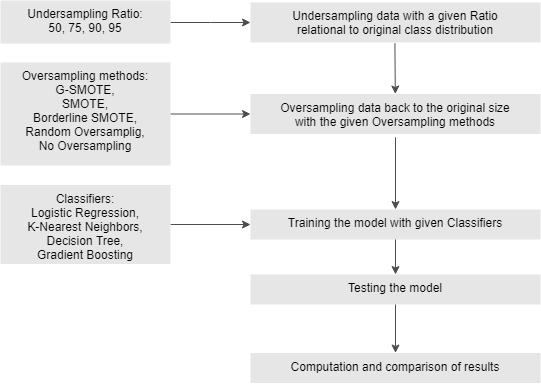
\includegraphics[width=0.7\linewidth]{resources/experimental_procedure}
	\caption{High-level experimental procedure}
	\label{fig:experimentalprocedure}
\end{figure}


We use $\mathit{k}$-fold cross-validation with $\mathit{k = 5}$ as a technique 
for assessing the performance of the models for each combination of oversampler 
and classifiers. The dataset $\mathit{D}$ is randomly split into $\mathit{k}$ 
subsets (folds) $\mathit{D_1, D_2, … D_k}$ of approximately equal size. Each 
fold is used as a validation set and the remaining folds are used to train the 
model with $\mathit{k}$ iterations. This procedure is repeated until each 
$\mathit{k}$ have been used as a validation set \cite{Han.2012}. Based on this 
technique, the experiment is conducted in the following steps within one 
iteration:

\begin{enumerate}
	\item 
	Splitting dataset into $\mathit{k}$-fold cross-validation sets where 
	$\mathit{k = 5}$
	\item 
	Undersampling $\mathit{k - 1}$ folds such that the class frequency remains 
	the same as the original with a ratio of 50, 75, 90 and 95 percent
	\item 
	Synthetic oversampling of $\mathit{k - 1}$ folds to the original size of 
	the dataset (class ratio remains the same) with G-SMOTE, SMOTE, Borderline 
	SMOTE, Random Oversampling and No Oversampling
	\item 
	Training the model with the classifiers LR, KNN, DT and GB
	\item 
	Testing the model with the remaining, original fold
	\item 
	Computation of results
\end{enumerate}	

This procedure is repeated three times and the on average highest cross 
validation score for each combination of dataset, classifier, oversampler and 
evaluation metric is reported.

In order to confirm the statistical significance of the experimental results, 
the Friedman test \cite{Sheldon.1996} as well as the Holms test 
\cite{JanezDemsar.2006} are applied. The Friedman test is a non-parametric 
procedure to test hypothesis on ordinal scaled variables. Additionally, it can 
also be applied with interval data when normality and homogeneity assumption 
does not hold. We use the Friedman test to evaluate the data generation 
algorithms on each dataset separately. Ranking scores are assigned to each 
oversampling method with scores of 1 to 5 for the best and worst performing 
methods, respectively. The procedure compares the average ranks of the 
algorithms under the null hypothesis, which states that the independent 
variable has no effect on the dependent variable. In our case, the null 
hypothesis assumes that all five algorithms show identical performance 
independent of the oversampling method and evaluation metric used. If the 
null-hypothesis is rejected to our favour, we proceed with the Holms test. The 
Holms test acts as a post-hoc test for the Friedman test for controlling the 
family-wise error rate when all algorithms are compared to a control method and 
not between themselves. This non-parametric test is very powerful in situations 
where we want to test whether a newly proposed method is better than existing 
ones. The control method in our case is the proposed G-SMOTE method and is 
tested under the null hypothesis whether G-SMOTE yields an improved performance 
over other oversampling methods.

\subsubsection{Software Implementation}

The implementation of the experimental procedure is based on Python programming 
language with the Scikit-Learn library 
\cite{PedregosaF.VaroquauxG.GramfortA.MichelV.ThirionB.GriselO.BlondelM.Prette.2011}.
All functions, algorithms, experiments and results reported are 
provided at \url{http://github.com/AlgoWit/publications}. They can be adjusted 
and implemented in comparative studies as the procedure is fully integrated 
with the Scikit-Learn ecosystem.    

\section{Results and Discussion}

In this section the performance of the different oversamplers and the results 
of the statistical tests are presented and analysed.

\subsection{Comparative Presentation}

The mean cross validation scores and the standard deviation values per 
classifier across all datasets are presented in Table 
\ref{tab:mean_sem_scores}. The scores are presented for each undersampling 
ratio to evaluate how the methods perform as the dataset size diminishes. We  
include the benchmark method that represents the original dataset without 
applying undersampling before training the algorithm. This sample set is seen 
as the ground truth of our experiments which is expected to obtain the best 
results by design.

\begin{center}
\begin{footnotesize}
\csvreader[
	longtable=lllllllll,
	table head=
	\toprule\mdseries Ratio & \mdseries Classifier & \mdseries Metric & \mdseries NONE & \mdseries 
	RANDOM & \mdseries SMOTE & \mdseries B-SMOTE & \mdseries G-SMOTE & \mdseries BENCHMARK \\
	\midrule\endhead
	\bottomrule\endfoot,
	late after line=\\,
	before reading={\catcode`\#12},
	after reading={\catcode`\#12},
	]{./resources/mean_sem_scores.csv}
	{1=\ratio,2=\classifier,3=\metric,4=\none,5=\random,6=\smote,7=\bsmote,
		8=\gsmote,9=\benchmark}
	{\ratio & \classifier & \metric & \none & \random & \smote & \bsmote & 	
	\gsmote & \benchmark}
\end{footnotesize}
\addtocounter{table}{-1}
\captionof{table}{Results for mean cross validation 
	scores of oversamplers (NONE corresponds to No Oversampling, RANDOM 
	to Random Oversampling and B-SMOTE to Borderline SMOTE)}
\label{tab:mean_sem_scores}
\end{center}

This table shows that G-SMOTE outperforms nearly all oversampling methods used 
for both, accuracy and G-mean metrics, on all classifiers. The highest score in 
the experiment is achieved by G-SMOTE with Gradient Boosting classifier and an 
average accuracy of 93\%. The undersampling ratio in this case is 50\% of the 
entire dataset. Throughout the scores we can observe that all oversamplers have 
a better performance as the dataset increase their size i.e. the undersampling 
ratio gets smaller. There is also a pattern in the performance of the 
classifiers. The better results a classifier can establish, the better the 
performance of the oversamplers in general. 

The scores of G-SMOTE are very similar to the ones of the Benchmark method 
which implies that the proposed method is able to artificially establish a 
representative dataset. Of all oversampling methods, the artificial data 
created by G-SMOTE is the one closest to the observed data of the benchmark 
method.

Table 3 presents the mean and standard error of percentage difference between 
G-SMOTE and SMOTE. It shows that G-SMOTE performs better on average than SMOTE 
in almost every combination of ratio, classifier and metric. 

\begin{center}
	\begin{footnotesize}
		\csvreader[
		longtable=llll,
		table head=
		\toprule\mdseries Ratio & \mdseries Classifier & \mdseries Metric & \mdseries Difference \\
		\midrule\endhead
		\bottomrule\endfoot,
		late after line=\\,
		before reading={\catcode`\#12},
		after reading={\catcode`\#12},
		]{./resources/mean_sem_perc_diff_scores.csv}
		{1=\ratio,2=\classifier,3=\metric,4=\difference}
		{\ratio & \classifier & \metric & \difference}
	\end{footnotesize}
	\addtocounter{table}{-1}
	\captionof{table}{Results for percentage difference between G-SMOTE and SMOTE}
	\label{tab:mean_sem_perc_diff_scores}
\end{center}

As explained in section 4, a ranking score in the range 1 to 5 is assigned to 
each oversampler. The mean ranking of all oversampling methods across the 
datasets is presented in the following figure: 

\begin{figure}[H]
	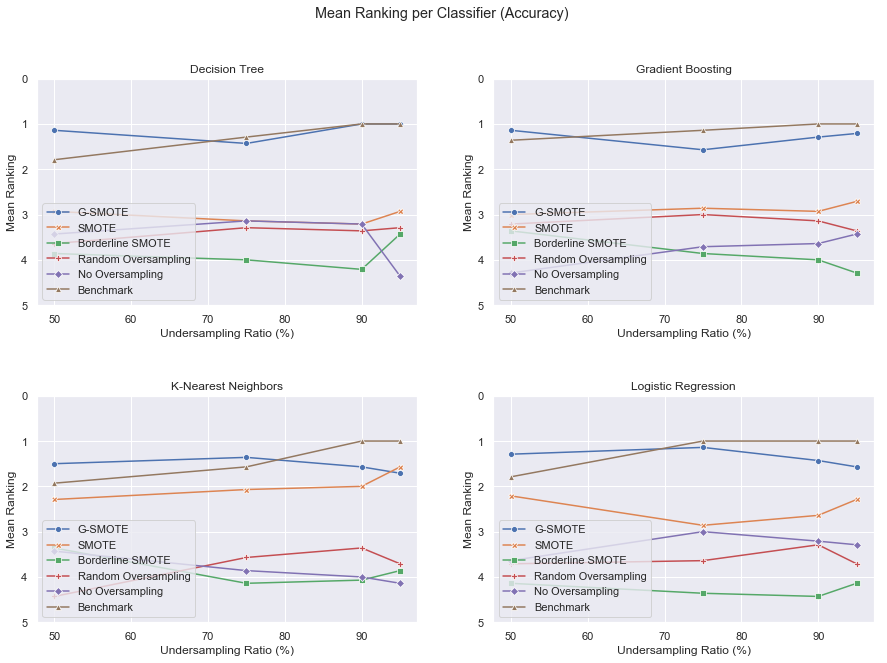
\includegraphics[width=1\linewidth]
		{resources/mean_ranking_per_classifier_accuracy}
	\caption{Mean ranking per classifier (Accuracy)}
	\label{fig:mean_ranking_per_classifier_accuracy}
\end{figure}

Looking at the graphs, G-SMOTE is ranked on the top place when comparing with 
SMOTE, Borderline SMOTE, Random Oversampling and No Oversampling. Additionally, 
G-SMOTE slightly outperforms the Benchmark method using the classifiers 
Logistic Regression and Decision Tree in the mean ranking. 

\subsection{Statistical Analysis}

To confirm the significance of the above presented results we apply the 
Friedman test as well as the Holms Test on our results. The application of the 
Friedman test shows the following results:

\begin{table}[H]
	\begin{tabular}{ll|ll|ll|ll|ll}
		&          & \multicolumn{2}{c|}{50\%} & \multicolumn{2}{c|}{75\%} & 
		\multicolumn{2}{c|}{90\%} & \multicolumn{2}{c}{95\%} \\
		\textbf{Classifier} & \textbf{Metric}   & \textbf{p-value}  & 
		\textbf{Sig}  & \textbf{p-value}   & 
		\textbf{Sig}  & \textbf{p-value}   & \textbf{Sig}  & 
		\textbf{p-value}   & \textbf{Sig}  
		\\ \hline
		LR         & Accuracy & 2.00E-03  & TRUE          & 2.80E-03  & 
		TRUE          & 9.30E-03  & TRUE          & 1.20E-02  & TRUE          \\
		LR         & G-Mean   & 3.30E-02  & TRUE          & 1.40E-02  & 
		TRUE          & 1.30E-02  & TRUE          & 7.30E-02  & FALSE         \\
		KNN        & Accuracy & 3.50E-03  & TRUE          & 2.20E-03  & 
		TRUE          & 4.70E-03  & TRUE          & 1.60E-03  & TRUE          \\
		KNN        & G-Mean   & 1.00E-02  & TRUE          & 9.30E-04  & 
		TRUE          & 2.00E-04  & TRUE          & 7.90E-03  & TRUE          \\
		DT         & Accuracy & 5.50E-03  & TRUE          & 1.90E-02  & 
		TRUE          & 1.80E-03  & TRUE          & 2.00E-04  & TRUE          \\
		DT         & G-Mean   & 2.20E-03  & TRUE          & 4.50E-02  & 
		TRUE          & 6.80E-03  & TRUE          & 1.40E-03  & TRUE          \\
		GBC        & Accuracy & 3.00E-03  & TRUE          & 2.90E-02  & 
		TRUE          & 6.10E-03  & TRUE          & 3.00E-03  & TRUE          \\
		GB        & G-Mean   & 3.40E-03  & TRUE          & 4.50E-02  & 
		TRUE          & 8.70E-03  & TRUE          & 2.40E-02  & TRUE         
	\end{tabular}
\caption{\label{tab:friedman-test}Results for Friedman test}
\end{table}

Therefore, the null hypothesis of the Friedman test is rejected at a 
significance level of a = 0.05, i.e. the classifiers do not perform similarly 
in the mean rankings across the oversampling methods and evaluation metrics.

[Holms test]

\section{Conclusions}

This research illustrates an effective solution to mitigate the small dataset 
problem in supervised learning tasks. The oversampling algorithm G-SMOTE has 
the ability to represent the underlying population of a small sample very well 
and is able to improve prediction accuracy on limited data for binary 
classification problems. This improvement in the forecasting performance of 
G-SMOTE relates to its capability of increasing the diversity of generated 
instances while generating artificial samples in safe areas of the input space. 
The successful implementation of this oversampler in imbalance data problems 
can be translated into small dataset problems, which shows a lot of potential 
for possible linkage of these research areas in the future. The G-SMOTE 
algorithm is available for implementation on GitHub 
(\url{https://github.com/AlgoWit/geometric-smote}) or 
\url{http://geometric-smote.readthedocs.io}.

\bibliography{references}
\bibliographystyle{apalike}

\end{document}
